\documentclass[12pt]{article}
%	options include 12pt or 11pt or 10pt
%	classes include article, report, book, letter, thesis

% \usepackage[margin=0.75in]{geometry}
\usepackage[margin=1in]{geometry}
\setlength{\parindent}{0pt}

\usepackage{hyperref}

%for writing of code in blocks like
%\begin{lstlisting}
%   .......
%\end{lstlisting}
\usepackage{listings}
\usepackage{color}
\usepackage{enumitem}
\usepackage{graphicx}

\definecolor{dkgreen}{rgb}{0,0.6,0}
\definecolor{gray}{rgb}{0.5,0.5,0.5}
\definecolor{mauve}{rgb}{0.58,0,0.82}

\lstset{frame=tb,
  language=C++,
  aboveskip=3mm,
  belowskip=3mm,
  showstringspaces=false,
  columns=flexible,
  basicstyle={\small\ttfamily},
  numbers=none,
  numberstyle=\tiny\color{gray},
  keywordstyle=\color{blue},
  commentstyle=\color{dkgreen},
  stringstyle=\color{mauve},
  breaklines=true,
  breakatwhitespace=true,
  tabsize=3
}
%%%%%%%%%%%%%%%%%%%%%%

\title{Life of a Particle : Quiz on Unit}
\author{Claire David}
\date{Due Date : 31/01/2019}

\begin{document}
\maketitle

% \textbf{Guidelines}: Choose one of the two quizzes below.

\section{The unit of charge: the Coulomb}
The elementary charge carried by the electron is $q_e = 1.6021766208(98) \times 10^{-19}$ C.\\
Do you know intuitively what is the charge in one Coulomb?

\begin{figure}[h]
    \centering
    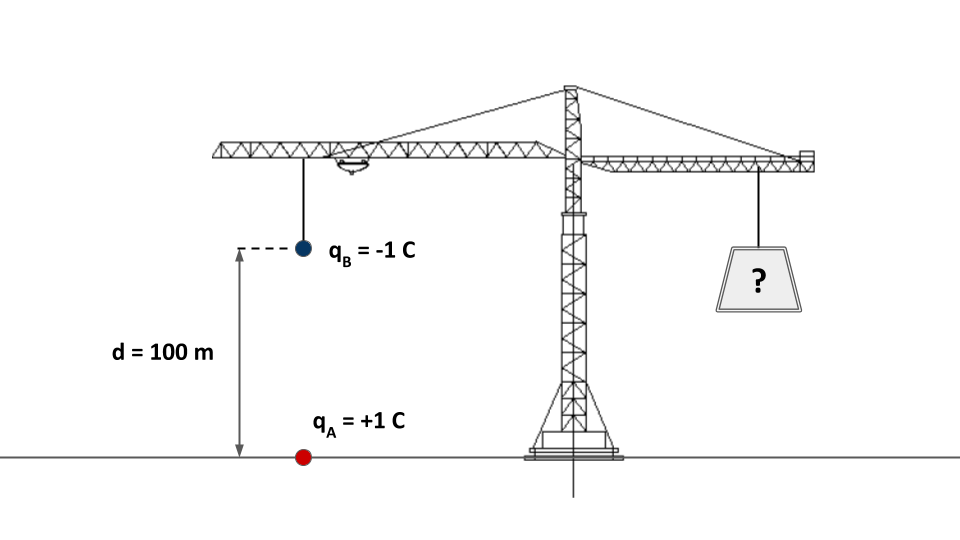
\includegraphics[width=0.85\textwidth]{Coulomb_quiz.png}
%     \caption{}
%     \label{fig:mesh1}
\end{figure}
Let's imagine we can fix a positive charge A of one Coulomb in the ground.\\
Let's have a crane where we hang a negative charge B of one Coulomb above the first at a distance $d = 100$ m.\\
The two charges will attract each other, according to the Coulomb force.\\


\textbf{Question A:} What is the mass to be suspended on the other side of the crane to balance this system out? Compare this to a day-to-day life object.\\



\textbf{Question B:} A typical lightning strike is about 40 coulombs of charge, typically consisting of four separate "strokes". (That's why lightning usually looks flickery.) Each stroke lasts about 30 microseconds. What is the current?\\



\textit{Reminder:}\\


Coulomb's law is given by:
\begin{equation}
 \mathbf{F_{12}} = k_e \frac{|q_1| \, |q_2|}{\mathbf{r_{21}}^2} \: \mathbf{\hat{r}_{21}} 
\end{equation}
with:
    \begin{description}
        \item $k_e$: Coulomb's constant, $k_e = 8.9875517873681764 \times 10^9$ N m$^2$ C$^{-2}$
        \item $q_i$: charge of object $i$
        \item $r$: distance between the charges
    \end{description}

\section{The electron volt}
An electron volt (eV) is the energy an electron gains when it is accelerated through a potential difference of one volt. An electron volt is defined as a unit of energy.\\

A Lindt 70\% cocoa chocolate bar has 194 Calories (one dietary Calorie, is 1000 calories, or 4184 Joules).\\

The LHC operates at 14 TeV (tera eV, 10$^{12}$ eV).\\


\textbf{Question A:} How does the LHC energy of the proton-proton collisions compare with respect to the energy stored in a cocoa chocolate bar?\\ 

\textbf{Question B:} Make the same comparison with energy density.\\

\vspace{4ex}
\hrule
\vspace{4ex}
\textit{Data:} as volumes you can use these estimations as guideline:
    \begin{description}
        \item LHC: a proton has a volume of roughly 1 fm$^3$, or about 10$^{-39}$ cm$^3$
        \item Lindt 70\% cocoa chocolate bar is about 10 cm $\times$ 1/2 cm $\times$ 20 cm = 100 cm$^3$
    \end{description}

\vspace{4ex}
\hrule
\vspace{4ex}
    
\end{document}